% Generated by eval/scripts/write_reference_comparison_figures.py.
\definecolor{srweak}{RGB}{35,103,159}
\definecolor{srstrong}{RGB}{202,86,42}
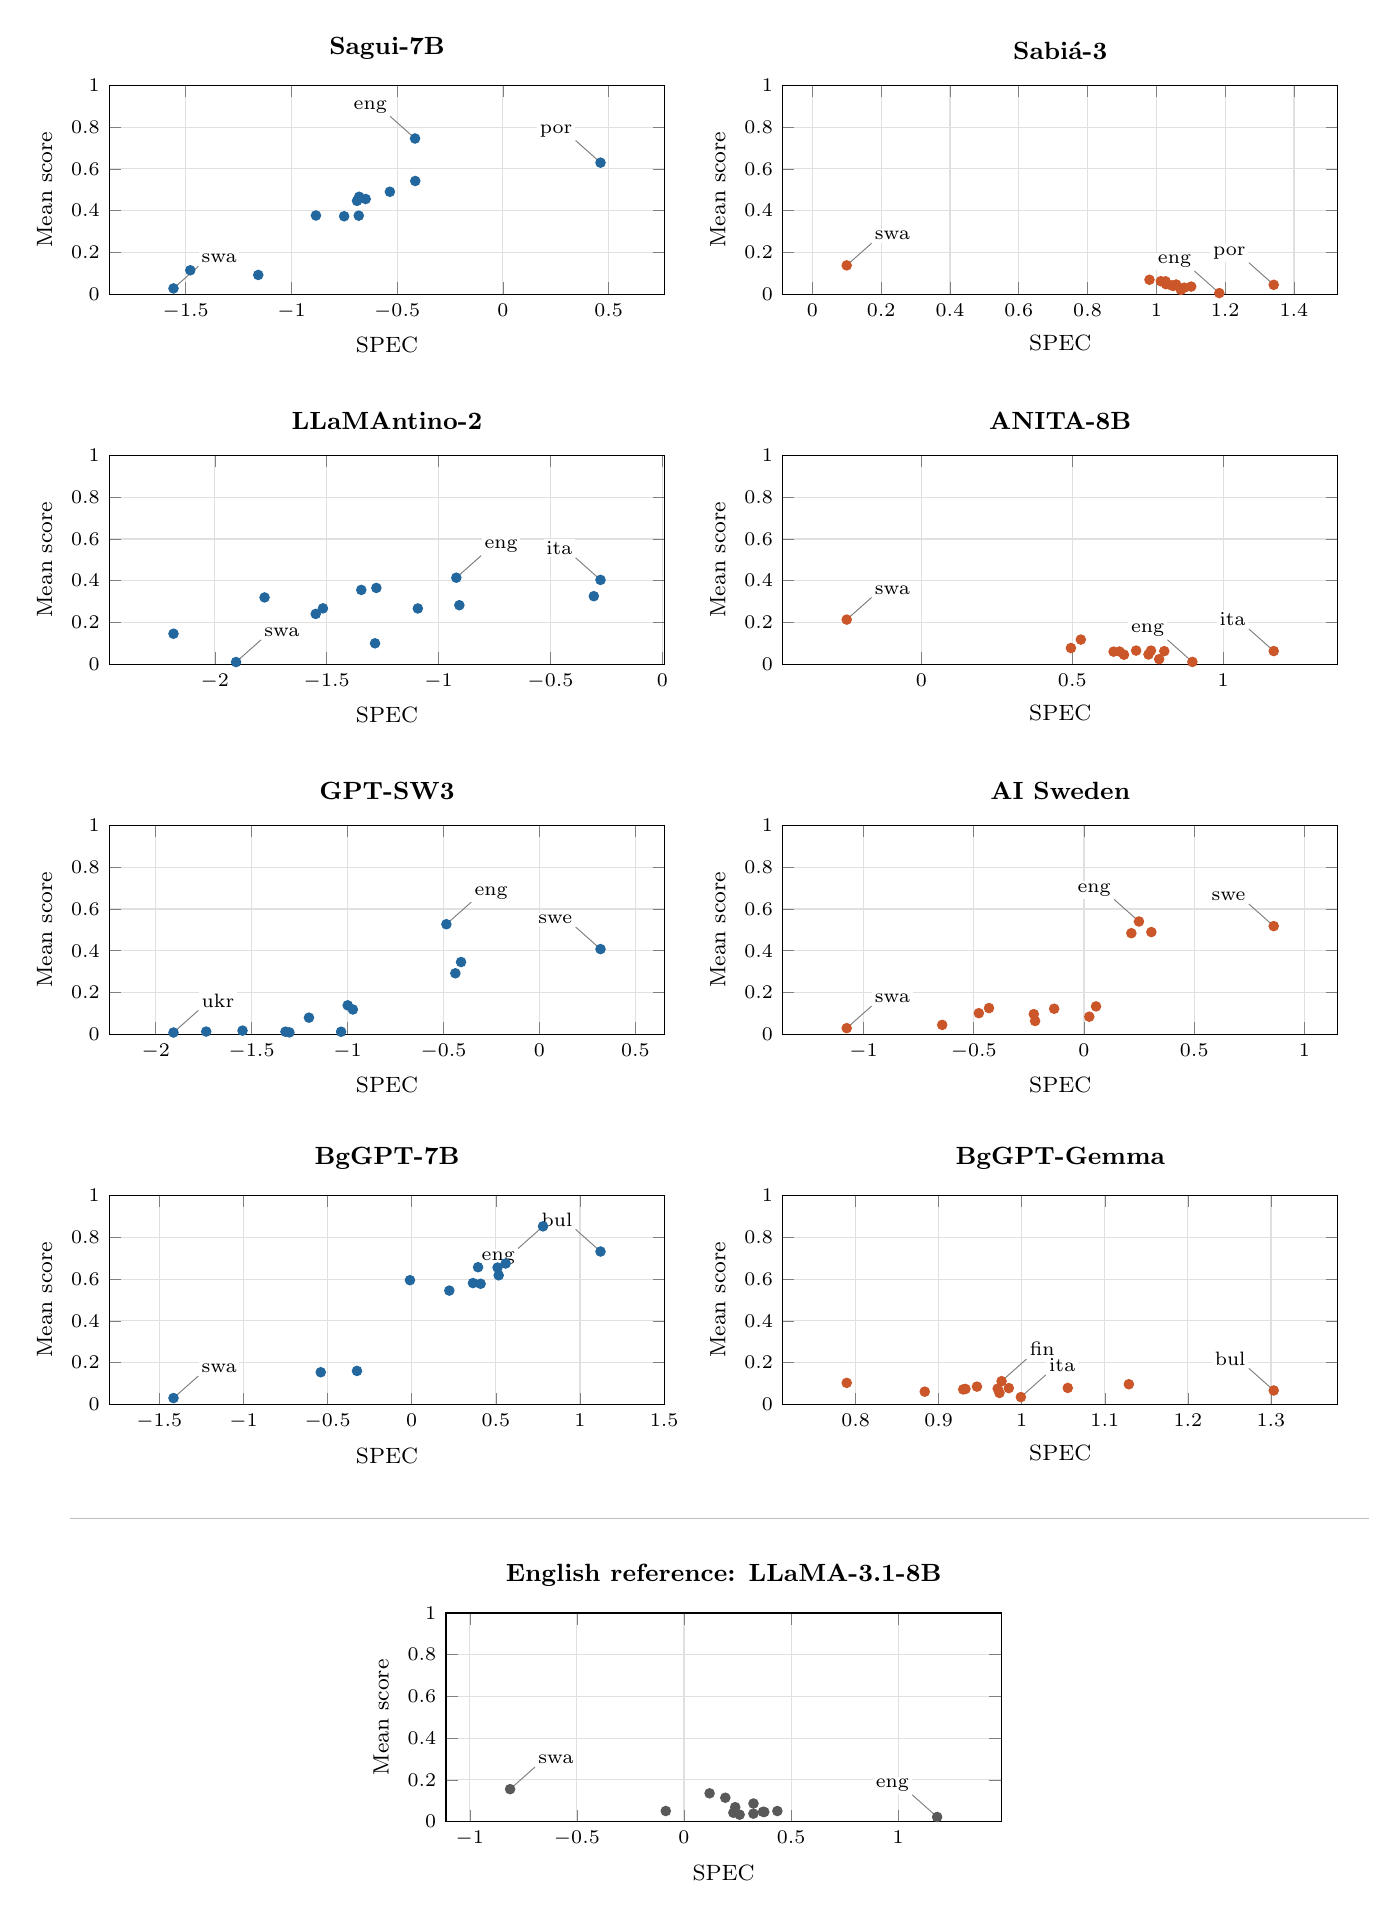
\begin{tikzpicture}
\pgfplotsset{srscatter/.style={width=7.05cm,height=2.65cm,scale only axis,ymin=0,ymax=1,ytick={0,.2,.4,.6,.8,1},xlabel={SPEC},ylabel={Mean score},axis lines=box,grid=major,grid style={black!12},tick label style={font=\scriptsize},label style={font=\footnotesize},title style={font=\bfseries\small},enlarge x limits=.15}}
\begin{axis}[srscatter,at={(0.0cm,-0.0cm)},anchor=north west,title={Sagui-7B}]
\addplot[only marks,color=srweak,mark=*,mark size=1.7pt] coordinates {(0.461719,0.629808) (-0.534344,0.490415) (-0.681593,0.375804) (-0.414341,0.541933) (-0.750621,0.372937) (-0.415355,0.745607) (-1.156874,0.091724) (-0.648837,0.455529) (-0.689740,0.446774) (-1.557684,0.027104) (-0.679633,0.466346) (-1.478279,0.114078) (-0.884044,0.376608)};
\node[font=\scriptsize,anchor=south east,xshift=-9pt,yshift=8pt,fill=white,inner sep=1pt] (languageLabel0) at (axis cs:0.461719,0.629808) {por};
\draw[black!50,line width=.35pt] (languageLabel0.south east) -- (axis cs:0.461719,0.629808);
\node[font=\scriptsize,anchor=south east,xshift=-9pt,yshift=8pt,fill=white,inner sep=1pt] (languageLabel1) at (axis cs:-0.415355,0.745607) {eng};
\draw[black!50,line width=.35pt] (languageLabel1.south east) -- (axis cs:-0.415355,0.745607);
\node[font=\scriptsize,anchor=south west,xshift=9pt,yshift=8pt,fill=white,inner sep=1pt] (languageLabel2) at (axis cs:-1.557684,0.027104) {swa};
\draw[black!50,line width=.35pt] (languageLabel2.south west) -- (axis cs:-1.557684,0.027104);
\end{axis}
\begin{axis}[srscatter,at={(8.55cm,-0.0cm)},anchor=north west,title={Sabi\'a-3}]
\addplot[only marks,color=srstrong,mark=*,mark size=1.7pt] coordinates {(1.341249,0.044471) (1.071393,0.019968) (1.057568,0.045820) (1.080968,0.030751) (1.049015,0.039191) (1.182979,0.004792) (0.980022,0.068686) (1.101309,0.036058) (1.012947,0.061694) (0.099809,0.137540) (1.044153,0.041935) (1.027922,0.047330) (1.026637,0.061093)};
\node[font=\scriptsize,anchor=south east,xshift=-9pt,yshift=8pt,fill=white,inner sep=1pt] (languageLabel0) at (axis cs:1.341249,0.044471) {por};
\draw[black!50,line width=.35pt] (languageLabel0.south east) -- (axis cs:1.341249,0.044471);
\node[font=\scriptsize,anchor=south east,xshift=-9pt,yshift=8pt,fill=white,inner sep=1pt] (languageLabel1) at (axis cs:1.182979,0.004792) {eng};
\draw[black!50,line width=.35pt] (languageLabel1.south east) -- (axis cs:1.182979,0.004792);
\node[font=\scriptsize,anchor=south west,xshift=9pt,yshift=8pt,fill=white,inner sep=1pt] (languageLabel2) at (axis cs:0.099809,0.137540) {swa};
\draw[black!50,line width=.35pt] (languageLabel2.south west) -- (axis cs:0.099809,0.137540);
\end{axis}
\begin{axis}[srscatter,at={(0.0cm,-4.7cm)},anchor=north west,title={LLaMAntino-2}]
\addplot[only marks,color=srweak,mark=*,mark size=1.7pt] coordinates {(-0.276208,0.403754) (-1.277911,0.365354) (-1.777672,0.319719) (-1.345337,0.355769) (-1.548931,0.240756) (-0.306124,0.325721) (-0.920645,0.414263) (-2.184595,0.145904) (-1.516673,0.267395) (-1.904936,0.010113) (-0.907046,0.282556) (-1.283832,0.099919) (-1.092590,0.266935)};
\node[font=\scriptsize,anchor=south east,xshift=-9pt,yshift=8pt,fill=white,inner sep=1pt] (languageLabel0) at (axis cs:-0.276208,0.403754) {ita};
\draw[black!50,line width=.35pt] (languageLabel0.south east) -- (axis cs:-0.276208,0.403754);
\node[font=\scriptsize,anchor=south west,xshift=9pt,yshift=8pt,fill=white,inner sep=1pt] (languageLabel1) at (axis cs:-0.920645,0.414263) {eng};
\draw[black!50,line width=.35pt] (languageLabel1.south west) -- (axis cs:-0.920645,0.414263);
\node[font=\scriptsize,anchor=south west,xshift=9pt,yshift=8pt,fill=white,inner sep=1pt] (languageLabel2) at (axis cs:-1.904936,0.010113) {swa};
\draw[black!50,line width=.35pt] (languageLabel2.south west) -- (axis cs:-1.904936,0.010113);
\end{axis}
\begin{axis}[srscatter,at={(8.55cm,-4.7cm)},anchor=north west,title={ANITA-8B}]
\addplot[only marks,color=srstrong,mark=*,mark size=1.7pt] coordinates {(1.167736,0.062700) (0.760839,0.064904) (0.671355,0.045380) (0.804886,0.062300) (0.711655,0.065113) (0.787907,0.024038) (0.898047,0.010783) (0.528236,0.117747) (0.752557,0.046371) (-0.247794,0.213592) (0.656386,0.060497) (0.495481,0.077265) (0.636848,0.059887)};
\node[font=\scriptsize,anchor=south east,xshift=-9pt,yshift=8pt,fill=white,inner sep=1pt] (languageLabel0) at (axis cs:1.167736,0.062700) {ita};
\draw[black!50,line width=.35pt] (languageLabel0.south east) -- (axis cs:1.167736,0.062700);
\node[font=\scriptsize,anchor=south east,xshift=-9pt,yshift=8pt,fill=white,inner sep=1pt] (languageLabel1) at (axis cs:0.898047,0.010783) {eng};
\draw[black!50,line width=.35pt] (languageLabel1.south east) -- (axis cs:0.898047,0.010783);
\node[font=\scriptsize,anchor=south west,xshift=9pt,yshift=8pt,fill=white,inner sep=1pt] (languageLabel2) at (axis cs:-0.247794,0.213592) {swa};
\draw[black!50,line width=.35pt] (languageLabel2.south west) -- (axis cs:-0.247794,0.213592);
\end{axis}
\begin{axis}[srscatter,at={(0.0cm,-9.4cm)},anchor=north west,title={GPT-SW3}]
\addplot[only marks,color=srweak,mark=*,mark size=1.7pt] coordinates {(0.318123,0.408065) (-0.438340,0.292067) (-0.408694,0.346061) (-1.033724,0.011945) (-0.485024,0.527157) (-0.972369,0.118590) (-1.547373,0.017283) (-1.907215,0.008251) (-1.201291,0.079473) (-1.736743,0.012821) (-0.999245,0.138578) (-1.323659,0.012136) (-1.303106,0.008900)};
\node[font=\scriptsize,anchor=south east,xshift=-9pt,yshift=8pt,fill=white,inner sep=1pt] (languageLabel0) at (axis cs:0.318123,0.408065) {swe};
\draw[black!50,line width=.35pt] (languageLabel0.south east) -- (axis cs:0.318123,0.408065);
\node[font=\scriptsize,anchor=south west,xshift=9pt,yshift=8pt,fill=white,inner sep=1pt] (languageLabel1) at (axis cs:-0.485024,0.527157) {eng};
\draw[black!50,line width=.35pt] (languageLabel1.south west) -- (axis cs:-0.485024,0.527157);
\node[font=\scriptsize,anchor=south west,xshift=9pt,yshift=8pt,fill=white,inner sep=1pt] (languageLabel2) at (axis cs:-1.907215,0.008251) {ukr};
\draw[black!50,line width=.35pt] (languageLabel2.south west) -- (axis cs:-1.907215,0.008251);
\end{axis}
\begin{axis}[srscatter,at={(8.55cm,-9.4cm)},anchor=north west,title={AI Sweden}]
\addplot[only marks,color=srstrong,mark=*,mark size=1.7pt] coordinates {(0.860599,0.518145) (0.305513,0.489583) (0.214828,0.484274) (-0.643025,0.044795) (0.249262,0.540335) (0.024003,0.084135) (-0.476834,0.100884) (-0.430727,0.125413) (-0.221643,0.063498) (-0.135220,0.122196) (0.054674,0.133387) (-0.227663,0.096278) (-1.076084,0.029126)};
\node[font=\scriptsize,anchor=south east,xshift=-9pt,yshift=8pt,fill=white,inner sep=1pt] (languageLabel0) at (axis cs:0.860599,0.518145) {swe};
\draw[black!50,line width=.35pt] (languageLabel0.south east) -- (axis cs:0.860599,0.518145);
\node[font=\scriptsize,anchor=south east,xshift=-9pt,yshift=8pt,fill=white,inner sep=1pt] (languageLabel1) at (axis cs:0.249262,0.540335) {eng};
\draw[black!50,line width=.35pt] (languageLabel1.south east) -- (axis cs:0.249262,0.540335);
\node[font=\scriptsize,anchor=south west,xshift=9pt,yshift=8pt,fill=white,inner sep=1pt] (languageLabel2) at (axis cs:-1.076084,0.029126) {swa};
\draw[black!50,line width=.35pt] (languageLabel2.south west) -- (axis cs:-1.076084,0.029126);
\end{axis}
\begin{axis}[srscatter,at={(0.0cm,-14.1cm)},anchor=north west,title={BgGPT-7B}]
\addplot[only marks,color=srweak,mark=*,mark size=1.7pt] coordinates {(1.121865,0.732315) (0.394273,0.657051) (0.516845,0.618189) (-0.325170,0.159983) (-0.010458,0.594884) (0.409383,0.577724) (0.510152,0.655351) (0.780344,0.853035) (0.558322,0.674920) (0.364052,0.581048) (-0.540499,0.153722) (0.223530,0.545016) (-1.415608,0.029935)};
\node[font=\scriptsize,anchor=south east,xshift=-9pt,yshift=8pt,fill=white,inner sep=1pt] (languageLabel0) at (axis cs:1.121865,0.732315) {bul};
\draw[black!50,line width=.35pt] (languageLabel0.south east) -- (axis cs:1.121865,0.732315);
\node[font=\scriptsize,anchor=north east,xshift=-9pt,yshift=-8pt,fill=white,inner sep=1pt] (languageLabel1) at (axis cs:0.780344,0.853035) {eng};
\draw[black!50,line width=.35pt] (languageLabel1.north east) -- (axis cs:0.780344,0.853035);
\node[font=\scriptsize,anchor=south west,xshift=9pt,yshift=8pt,fill=white,inner sep=1pt] (languageLabel2) at (axis cs:-1.415608,0.029935) {swa};
\draw[black!50,line width=.35pt] (languageLabel2.south west) -- (axis cs:-1.415608,0.029935);
\end{axis}
\begin{axis}[srscatter,at={(8.55cm,-14.1cm)},anchor=north west,title={BgGPT-Gemma}]
\addplot[only marks,color=srstrong,mark=*,mark size=1.7pt] coordinates {(1.303355,0.066318) (0.973194,0.054487) (0.984450,0.077724) (0.975763,0.110922) (0.929587,0.071370) (1.055438,0.078526) (0.998986,0.034744) (1.128961,0.096246) (0.971064,0.075080) (0.932291,0.073651) (0.883276,0.060680) (0.946117,0.084807) (0.789336,0.102751)};
\node[font=\scriptsize,anchor=south east,xshift=-9pt,yshift=8pt,fill=white,inner sep=1pt] (languageLabel0) at (axis cs:1.303355,0.066318) {bul};
\draw[black!50,line width=.35pt] (languageLabel0.south east) -- (axis cs:1.303355,0.066318);
\node[font=\scriptsize,anchor=south west,xshift=9pt,yshift=8pt,fill=white,inner sep=1pt] (languageLabel1) at (axis cs:0.975763,0.110922) {fin};
\draw[black!50,line width=.35pt] (languageLabel1.south west) -- (axis cs:0.975763,0.110922);
\node[font=\scriptsize,anchor=south west,xshift=9pt,yshift=8pt,fill=white,inner sep=1pt] (languageLabel2) at (axis cs:0.998986,0.034744) {ita};
\draw[black!50,line width=.35pt] (languageLabel2.south west) -- (axis cs:0.998986,0.034744);
\end{axis}
\draw[black!25] (-.5,-18.2) -- (16,-18.2);
\begin{axis}[srscatter,at={(4.275cm,-19.4cm)},anchor=north west,title={English reference: LLaMA-3.1-8B}]
\addplot[only marks,color=black!65,mark=*,mark size=1.7pt] coordinates {(1.181697,0.022364) (0.324334,0.086939) (0.239115,0.069311) (0.368920,0.047026) (0.374768,0.046371) (0.192872,0.114550) (0.259633,0.033416) (0.324048,0.038339) (0.119382,0.135666) (0.230438,0.042732) (-0.084995,0.050971) (0.435809,0.050881) (-0.811875,0.155744)};
\node[font=\scriptsize,anchor=south east,xshift=-9pt,yshift=8pt,fill=white,inner sep=1pt] (languageLabel0) at (axis cs:1.181697,0.022364) {eng};
\draw[black!50,line width=.35pt] (languageLabel0.south east) -- (axis cs:1.181697,0.022364);
\node[font=\scriptsize,anchor=south west,xshift=9pt,yshift=8pt,fill=white,inner sep=1pt] (languageLabel1) at (axis cs:-0.811875,0.155744) {swa};
\draw[black!50,line width=.35pt] (languageLabel1.south west) -- (axis cs:-0.811875,0.155744);
\end{axis}
\end{tikzpicture}
